\chapter{NDT SLAM problem analysis}

The full \gls{SLAM} problem solution requires a combination of data association, mapping and pose estimation.
In the first step, the algorithm needs to receive data from sensors. The standard SLAM requires information about the movement of the robot and robot's perception of an environment.  The standard odometry tracking of the robot is done with wheel encoders or with the \gls{IMU}.Perception of the environment can be obtained from 2D or 3D laser scanner. Another option is to use stereo cameras or Kinect\footnote{\url{www.xbox.com/en-US/kinect}}.  

\gls{SLAM} algorithm based on laser scans are still frequently used in real life applications. The standard versions work with 2D scans \cite{Hector} \cite{gmapping}. Two scans can be used for a registration. It is a process which calculates relative transformation between two scans by aligning one scan on top of the other one. The registration is used for a variety of tasks, e.g. map building, odometry estimation, unique feature detection. Some registration techniques are described in the section \ref{sec:Scan_reg}.

The result of every \gls{SLAM} solution should be a map which can be used in navigation and a trajectory planning. One possible map representation is the set of unique landmarks. The other option is to integrate measurement together and create a dense map of the environment. These methods will be analyzed in the section \ref{MAP_REPRE}

Lastly, we need to estimate a position of the robot based on information from odometry and the map. Hence, we need to define what it is the position of the robot and how we will represent it.
\section{SLAM problem definition}
\label{sec:SLAM_def}
We describe the position estimation problem as a process which finds the location of the robot in every time step. We also need to estimate how the map will look like in every time step. In the real world, we deal with the sensors which always have some inherited noise. Therefore, we are not able to provide exact position of the robot. For this reason, we use a probabilistic definition of the problem. The robot moves through unknown space along trajectory expressed as variables $ \textbf{x}_{1:T} = \{\textbf{x}_{1},...,\textbf{x}_{T}\} $. While moving robot is taking the odometry measurements $ \textbf{u}_{1:T} = \{\textbf{u}_{1},...,\textbf{u}_{T}\}$ and the perception of environment $ \textbf{z}_{1:T} = \{\textbf{z}_{1},...,\textbf{z}_{T}\}$. The solution to position estimation is a probability of the robot's trajectory $ \textbf{x}_{1:T}$ and the map \textbf{m} of the local environment given all the measurements and the initial pose $ \textbf{x}_{0}$:
\begin{equation}
p(\textbf{x}_{1:T}, \textbf{m}\: |\:  \textbf{z}_{1:T}, \textbf{u}_{1:T}, \textbf{x}_{0})
\end{equation}
The odometry is represented as triple $(x,y,\theta)$ in 2D system. The initial pose can be interpreted as an origin of the coordinate system for the global map.

\section{SLAM's position estimation categories}
Over the past decade researchers have developed three distinctive categories of \gls{SLAM} position estimation. 

The first type is the \gls{EKF} variant. It is based on the \gls{KF}. The \gls{KF}  assume that probability density function is from Gaussian distributions and the position model is linear. This assumption is usually not correct for the robot movement model. The \gls{EKF} solves the problem with non-linearity of the robot's pose model. The performance of \gls{EKF} strongly depends on a quality of statistical model for noise in the sensors and the odometry. Unfortunately, these models are usually not available. A set of comparative tests for convergence and inconsistencies of \gls{EKF} is in work of \cite{EKF}.

Another category is based on the \gls{PF}. The set of weighted particles represents the current state of the robot. This representation has the advantage in modeling uncertainty through a multi-modal distribution and can deal with non-Gaussian sensor noise. The authors \cite{FastSlam} proposed computationally efficient method based on the \gls{PF} called FastSLAM. It uses the particles to represent posterior probability of the robot motion. Each particle also holds K Kallman filters representing landmark positions (unique features in the environment). The authors of this algorithm have demonstrated that it is possible to calculate high-precision maps utilizing FastSLAM. Inspired by FastSlam, a method based on Rao-Blackwellized Particle Filter is proposed in \cite{Rao-PF}. Derivations of this approach are still actively used in robotics today.\cite{gmapping} 

The last category models positions of the robot with a graph representation.  The least square optimization of the graph finds a possible robot trajectory over time. A graph node represents a possible pose of the robot and an edge between two nodes is a relative movement. The Nodes may also hold some information about current state of the map or a laser measurement. This representation was first time used in work of \cite{LuMilios}. This technique was later improved by \cite{OlsonGS}. They have presented an efficient optimization approach based on the scholastic gradient descent. It was able to correct even large graphs. Later, multiple authors have improved \gls{SLAM} optimization by adding hierarchies to large graphs or adding robustness to the optimization process. The graph-based model of SLAM offers flexibility for adaptation of new improvements and can be reasonably fast even on large graphs. More details about a graph generation and optimization is in the section \ref{sec:graph_base_slam}.

\section {Map representation}
\label{MAP_REPRE}
A map of an unknown environment is a standard part of the SLAM problem solution. This map needs to be stored for local path planning and obstacle avoidance. The map precision is an important characteristic for an obstacle avoidance algorithms. The ideal map should keep low memory consumption because robots often have limited access to memory.  The high-quality map is also beneficial for a precision of registration algorithms.

A point-cloud \cite{pcl} is the map representation which stores measurements as simple points in space. It is the most accurate representation because no data from the sensor are lost. Scan-matching algorithms e.g. \gls{ICP} use this data-structure. It is very easy to convert from this model to a different type of a map because it has all the information from the sensor measurement. A Problem is a memory consumption. If the robot runs for a long time with a higher frequency of the sensor data production, it is likely that robot will consume a significant amount of memory.

An occupancy map is a grid-based type of the map. It consists of the grid with cells. In every cell, it has just one value describing the likelihood that cell is occupied. This value becomes higher with more incoming data measurements. It has a constant memory consumption over time. It is also possible to use this representation for the registration \cite{Hector}. Furthermore, it can represent unoccupied spaces with a low likelihood value. This feature is used by many path planning and obstacle avoidance algorithms.  The occupancy maps are the main output format for SLAM maps in ROS. 

A quadtree is a tree data structure. Each node of the tree has exactly four children. The nodes are decomposing space into smaller sub-areas. Every node has its threshold. When it is reached, the cell is divided into a four smaller cells. This process dynamically changes a resolution of the grid. Therefore, we get higher precision in places where it matters more. The maximal precision is bounded by the minimal size of leaf nodes.

The \gls{NDT} representation \cite{Biber03} uses grid-based data-structure. Each cell has normal distribution parameters stored inside. The normal distribution is calculated from scan points which are mapped into the cell. This model offers constant memory consumption over time. The \gls{NDT} has a better internal representation of the mapped points than octree (3D case of quad-tree) which was proven in the work of \cite{Saarinen13}. They have shown that a coarser \gls{NDT} grid can have a better map precision than finer octree map. The standard \gls{NDT} representation of the map is fully explained in the section \ref{subsec:NDT_grid}. The \gls{NDT} maps can also include occupancy information. This extension is called \gls{NDT-OM} and it is presented in the section \ref{subsec:NDT_OM}. Furthermore, this extension can remove dynamic objects from the map which is crucial for \gls{SLAM} in dynamic environment.      
\begin{figure}
	\centering
	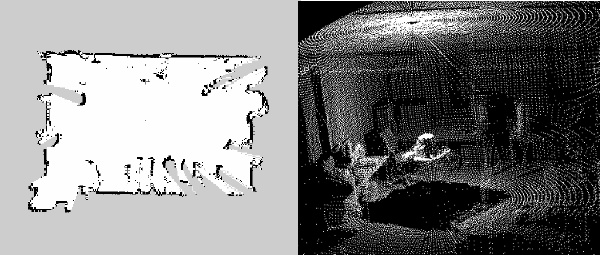
\includegraphics[width=100mm]{../img/maps.png}
	\caption{On the left is visualization of occupancy grid. On the right is visualized point cloud of a room.}
	\label{fig:maps}
\end{figure}
\newpage

\section{Registration}
\label{sec:Scan_reg}

A scan registration is a key concept in the full \gls{SLAM} solution. The \gls{SLAM} algorithm can use scan matching between two scans to determine a transformation. It tells us how far a robot moved between two scans. Unfortunately, these scans might not offer enough information for successful registration. Imagine a robot which is standing in the corner of a room with the sensor facing the wall. Scan from this robot has only information from a very limited field of view which may lead to alignment errors. Therefore, it is usually necessary to combine individual scans to operate with more data.  

One of the algorithms which use this process is called incremental scan-matching. It takes arriving scan and tries to match it against the map built from previous measurements. By doing so, it can be used as a replacement for robot odometry. The section \ref{subsec:D2D_NDT} provides the \gls{NDT} based algorithms which are suitable for incremental scan-matching. Another popular approach is the \gls{ICP} \cite{LuMilios}. All these algorithms use optimization methods (e.g. Newton's method) which require a good initial guess. Otherwise, they converge to some local minimum. 

The scan registration also verifies loop closures in the graph based \gls{SLAM}. The Loop closure is an edge which close the loop (creates a cycle) of robot's movement in the graph. More details about loop closure generation are in the section \ref{subsec:loop_closure_creation}. 

The scan matcher needs two scans to perform registration. The graph-based \gls{SLAM} stores these measurements inside of the nodes. In case that two nodes physically overlap they share the same measurement of the environment. The registration finds this similarity and calculates transformation between nodes. The biggest problem with this alignment is that we have no valid prior information about positions of these nodes. These two scans can overlap, or they can be from completely different parts of the world. The registration needs to estimate the transformation. Additionally, it needs to correctly identify if two scans overlap. We present one such an algorithm in the section \ref{subsec:Corr}    

\begin{figure}
\centering
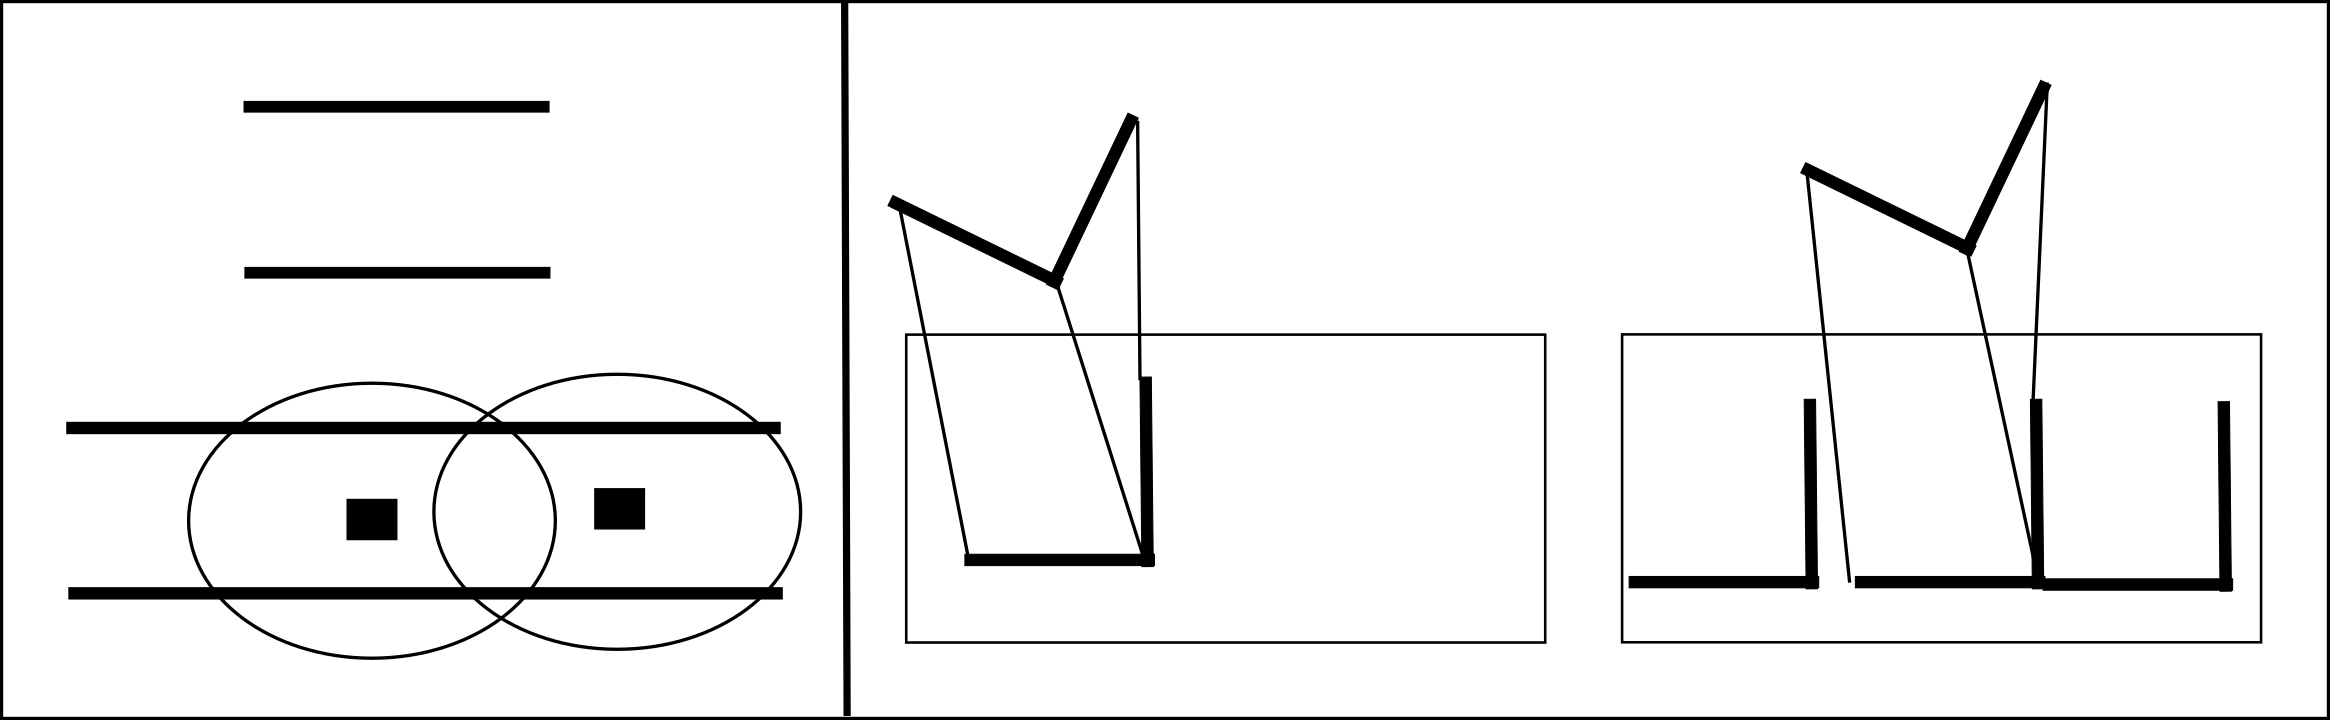
\includegraphics[width=100mm]{../img/ambi.png} 	
\caption{Local and global ambiguities in scan registrations. On the left is local ambiguity. On the right is global ambiguity with two maps. First map is original map without all information about environment. Second map is reality with all features. Registration wrongly associated matching based on information only from first map.} \label{fig:ambig}

\end{figure}

However, even scan matcher with correct validation can fail to identify the overlap. This is caused by ambiguities in the environment \cite{Olson2009Loop}.

The first is a local ambiguity.  Imagine a robot which moves in a long corridor similar to one in the figure \ref{fig:ambig} on the left. This environment does not have many distinctive features. One of the nodes has a measurement of two straight lines shown in top part. The second node has a measurement of the whole corridor shown on the bottom. The ellipses represent two out of an infinite number of correct alignments which would result in a perfect match. In reality, only one of them may be correct. Unfortunately, registration is not able to recognize the correct answer.

The second one is a global ambiguity. This ambiguity usually happens when the algorithm does not have enough information about the whole environment. One of the nodes has a measurement in the top part of the figure \ref{fig:ambig} on the right.  The second node has only information in the first rectangle. From this perspective, it looks like there is only one possible match. Unfortunately,  based on reality in the environment these two nodes do not overlap at all because the correct match is shown in the second rectangle.   Once again registration algorithm had no chance of figuring this out without prior knowledge about the whole environment.




  
\section {Graph-based SLAM on NDT maps}


After initial research, we have noticed benefits of the \gls{NDT} mapping. The \gls{NDT} maps have a good memory consumption. They can hold occupancy information and reject dynamic objects with the use of \gls{NDT-OM} extension \ref{subsec:NDT_OM}. The registration algorithms for the \gls{NDT} grids already exist. Unfortunately, they need initial guess for correct convergence. 

The Graph based pose estimation currently represent a flexible way how to find robot's position. It is also possible to extend it to work on large scale maps. Additional topological information from the graph can be beneficial for the detection of registration ambiguities.

Further, in the work of \cite{NDTOMFusion}, authors have described that scan matching based on the \gls{NDT} grids can provide precise result in mapping process with use of the \gls{NDT-OM} extension. They have proven this by mapping large area with the incremental scan matching. This process resulted in the precise map. They have noted in the conclusion that even though results are very accurate, there is a need for a solution with loop closure mechanism to improve results. They have also tested the reliability of dynamic object rejection. Their results have proven that the \gls{NDT-OM} is a really good option for a dynamic environment.

The loop closures can be created in graph based \gls{SLAM} and additionally tested by robust scan matcher. This work presents robust registration method for loop closure registration and validation on \gls{NDT} maps \ref{sec:Robust D2D-NDT}.

In the previous works, there was always one global \gls{NDT} map. The iterative scan matching then used this map for the alignment of incoming scans. In this work, we use the pose graph which is optimized by \gls{SLAM}'s back-end. The optimization makes changes to the location of the nodes which needs to update the global map. Therefore, we present a way how to represent the map which can be updated after graph optimization \ref{sec:NDT_frame}.

Incremental scan matching on \gls{NDT} grids was proven to get good results. Therefore, it should be included in this work as well and combine it with rest of the proposed system \ref{sec:window}.   

Lastly, it needs to be implemented in a way that on-line processing of real datasets is possible. It needs to have standard \gls{ROS} interface commonly found in other \gls{SLAM} packages. It should use standard libraries available in \gls{ROS}.

The final result of this works should be an implementation of 2D graph based \gls{SLAM} on \gls{NDT} maps with easy use inside of \gls{ROS} ecosystem. 